\section{Evaluation} \label{sec:eval}
We compare FIPS against the two groups that existing IEEE 802.1Qbv scheduling techniques fall into: \textit{non-robust} and \textit{strict transmission isolation} approaches.
Section~\ref{sec:eval:non-robust} shows that, compared to non-robust approaches, FIPS can serve a high-criticality stream with a $\qty{99.99}{\percent}$ reliability requirement.
Section~\ref{sec:eval:sti} shows that strict transmission isolation leads to poor scalability, whereas FIPS improves the number of schedulable wireless streams by up to $\times 45$.

\begin{figure}[t]
    \centering
    \resizebox{0.975\columnwidth}{!}{%
    \begin{tikzpicture}
	\node[inner sep=1pt] (L0) at (-1.3,0) {\includegraphics[width=0.5cm]{switch.png}} [thick, clockwise from=115, sibling angle=-130] 
	      child { node[inner sep=1pt] (L1) {\includegraphics[width=0.5cm]{switch.png}} [clockwise from=155, sibling angle=-50] 
		  child { node[inner sep=1pt] (L3) {\includegraphics[width=0.5cm]{card.png}} }
		  child { node[inner sep=1pt] (L4) {\includegraphics[width=0.5cm]{card.png}} }
	      }
	      child { node[inner sep=1pt] (L2) {\includegraphics[width=0.5cm]{switch.png}} [clockwise from=155, sibling angle=-50] 
		  child { node[inner sep=1pt] (L5) {\includegraphics[width=0.5cm]{card.png}} }
		  child { node[inner sep=1pt] (L6) {\includegraphics[width=0.5cm]{card.png}} }
	      };
	\draw[thick] (L1) edge (L2);

	\node[inner sep=1pt] (DetCom) at (0,0.1) {\includegraphics[width=0.4cm]{antennatower.png}};
	\node[font=\footnotesize,black!50,align=center] at (0,0.8) {Logical\\5G Bridge};

	\node[inner sep=1pt] (R0) at (1.3,0) {\includegraphics[width=0.5cm]{switch.png}} [thick, clockwise from=65, sibling angle=130] 
	    child { node[inner sep=1pt] (R1) {\includegraphics[width=0.5cm]{switch.png}} [clockwise from=25, sibling angle=50] 
		child { node[inner sep=1pt] (R3) {\includegraphics[width=0.5cm]{switch.png}} [clockwise from=15, sibling angle=30] 
		    child { node[inner sep=1pt] (R7) {\includegraphics[width=0.5cm]{card.png}} }
		    child { node[inner sep=1pt] (R8) {\includegraphics[width=0.5cm]{card.png}} }
		}
		child { node[inner sep=1pt] (R4) {\includegraphics[width=0.5cm]{switch.png}} [clockwise from=15, sibling angle=30] 
		    child { node[inner sep=1pt] (R9) {\includegraphics[width=0.5cm]{card.png}} }
		    child { node[inner sep=1pt] (R10) {\includegraphics[width=0.5cm]{card.png}} }
		}
	    }
	    child { node[inner sep=1pt] (R2) {\includegraphics[width=0.5cm]{switch.png}} [clockwise from=25, sibling angle=50] 
		child { node[inner sep=1pt] (R5) {\includegraphics[width=0.5cm]{switch.png}} [clockwise from=15, sibling angle=30] 
		    child { node[inner sep=1pt] (R11) {\includegraphics[width=0.5cm]{card.png}} }
		    child { node[inner sep=1pt] (R12) {\includegraphics[width=0.5cm]{card.png}} }
		}
		child { node[inner sep=1pt] (R6) {\includegraphics[width=0.5cm]{switch.png}} [clockwise from=15, sibling angle=30] 
		    child { node[inner sep=1pt] (R13) {\includegraphics[width=0.5cm]{card.png}} }
		    child { node[inner sep=1pt] (R14) {\includegraphics[width=0.5cm]{card.png}} }
		}
	    };
	\draw[thick] (R1) edge (R2);

	\draw[thick] (L0) edge (L0-|DetCom.west);
	\draw[thick] (R0) edge (R0-|DetCom.east);
	\node[font=\small,black!50] (AGV) at (-1.5,-2.1) {AGV};
	\node[font=\small,black!50] (Core) at (1.5,-2.4) {TSN Backbone};

	\begin{pgfonlayer}{background}
	  \node[draw, black!40, loosely dashed, rounded corners, fit={(L0) (L3) (L6) (AGV)}, inner sep=7pt] {};
	  \node[draw, black!40, loosely dashed, rounded corners, fit={(R0) (R7) (R14) (Core)}, inner sep=7pt] {};
	  \draw[black!40, fill=white] (0,0.1) ellipse (1.78cm and 1.1cm);
	\end{pgfonlayer}

	% wireless traffic
	\draw (L4) edge[-{Stealth[length=2mm]}, dashed, black!60, bend left=6mm] (L1);
	\draw (L1) edge[-{Stealth[length=2mm]}, dashed, black!60, bend left=6mm] (L0);
	\draw (L0) edge[-{Stealth[length=2mm]}, dashed, black!60, bend left=6mm] (DetCom);
	\draw (DetCom) edge[-{Stealth[length=2mm]}, dashed, black!60, bend left=6mm] (R0);
	\draw (R0) edge[-{Stealth[length=2mm]}, dashed, black!60, bend left=6mm] (R2);
	\draw (R2) edge[-{Stealth[length=2mm]}, dashed, black!60, bend left=6mm] (R5);
	\draw (R5) edge[-{Stealth[length=2mm]}, dashed, black!60, bend left=6mm] (R11);

	\draw (R8) edge[-{Stealth[length=2mm,open]}, dashed, black!60, bend left=6mm] (R3);
	\draw (R3) edge[-{Stealth[length=2mm,open]}, dashed, black!60, bend left=6mm] (R1);
	\draw (R1) edge[-{Stealth[length=2mm,open]}, dashed, black!60, bend left=6mm] (R0);
	\draw (R0) edge[-{Stealth[length=2mm,open]}, dashed, black!60, bend left=6mm, in=150, out=30] (DetCom);
	\draw (DetCom) edge[-{Stealth[length=2mm,open]}, dashed, black!60, bend left=6mm,out=30,in=150] (L0);
	\draw (L0) edge[-{Stealth[length=2mm,open]}, dashed, black!60, bend left=6mm] (L2);
	\draw (L2) edge[-{Stealth[length=2mm,open]}, dashed, black!60, bend left=6mm] (L5);

	% wireline traffic
	\draw (L4) edge[-{Stealth[length=2mm]}, black!60, bend right=6mm] (L1);
	\draw (L1) edge[-{Stealth[length=2mm]}, black!60, bend right=6mm] (L2);
	\draw (L2) edge[-{Stealth[length=2mm]}, black!60, bend right=6mm] (L5);

	\draw (R8) edge[-{Stealth[length=2mm,open]}, black!60, bend right=6mm] (R3);
	\draw (R3) edge[-{Stealth[length=2mm,open]}, black!60, bend right=6mm] (R1);
	\draw (R1) edge[-{Stealth[length=2mm,open]}, black!60, bend left=6mm] (R2);
	\draw (R2) edge[-{Stealth[length=2mm,open]}, black!60, bend right=6mm] (R5);
	\draw (R5) edge[-{Stealth[length=2mm,open]}, black!60, bend right=6mm] (R11);

	\draw (-3.7, 3) edge[-{Stealth[length=2mm,open]},black!60] (-3.2,3);
	\draw (-3, 3) edge[-{Stealth[length=2mm]},black!60] (-2.5,3);
	\node[font=\scriptsize] at (-3.1, 2.8) {wired streams};

	\draw (-1.9, 3) edge[-{Stealth[length=2mm,open]},black!60,dashed] (-1.4,3);
	\draw (-1.2, 3) edge[-{Stealth[length=2mm]},black!60,dashed] (-0.7,3);
	\node[font=\scriptsize] at (-1.3, 2.8) {wireless streams};

	\node[black!50, font=\tiny, fill=white, inner sep=1pt] at (-1.3,-0.3) {DS-TT};
	\node[black!50, font=\tiny, fill=white, inner sep=1pt] at (1.3,-0.3) {NW-TT};
    \end{tikzpicture}
    }
    \caption{Network simulating a simple industrial AGV use case.} \label{fig:eval_topology}
\end{figure}



\subsection{Methodology}
We simulate an automated guided vehicle~(AGV) as part of a networked control system.
To this end, we use the OMNeT++ simulation framework~\cite{Varga2010}, including the INET~\cite{Mros2019} and 6GDetCom~\cite{lucas_2023_10401977} extensions.
As shown in Fig.~\ref{fig:eval_topology}, the network is partitioned into the AGV-internal network and the TSN backbone.
Internal TSN devices and switches are connected by $\qty{100}{\mega\bit\per\s}$ Ethernet links with a propagation delay of $\qty{50}{\ns}$. 
The partitions are interconnected by a logical 5G bridge with uplink (DS-TT to NW-TT) and downlink (NW-TT to DS-TT) histograms taken from real 5G measurements \cite{downlink_example_histogram}.

We differentiate between wired and wireless traffic. 
Wired traffic stays within the AGV-internal network or the TSN backbone, with specifications $\size{F} = \qty{100}{\byte}$, $\period{F} = \qty{5}{\ms}$, $\ete{f} = \qty{500}{\us}$, and $\jitter{f} = \qty{1}{\us}$.
Wireless traffic traverses the logical 5G bridge in uplink or downlink direction, with specifications $\size{F} = \qty{100}{\byte}$ and $\period{F} = \qty{20}{\ms}$.
Depending on the evaluated scenario, we consider different QoS requirements for wireless streams.

All computations (simulation and scheduling) are performed on the same machine, equipped with two AMD EPYC 7413 @\qty{3.6}{\giga\hertz} ($2\times24$ cores) and with $\qty{256}{\giga\byte}$ of memory.
\textit{To facilitate reproducibility, we will publish the source code and Docker images for each benchmark once the paper is accepted.}

\subsection{Comparing FIPS with Non-Robust Approaches} \label{sec:eval:non-robust}
To illustrate the importance of robust end-to-end scheduling, we compare the achieved QoS of FIPS and non-robust scheduling approaches.
As existing work typically considers scalar 5G packet delays~\cite{9212049,9940254}, we compare FIPS to using the median (MED) or the maximum (MAX) 5G packet delays from the histograms.

% Results are provided in simulation_results.log
\begin{figure}
  \centering
  \begin{subfigure}{0.48\columnwidth}
    \centering
      \resizebox{\textwidth}{!}{%
      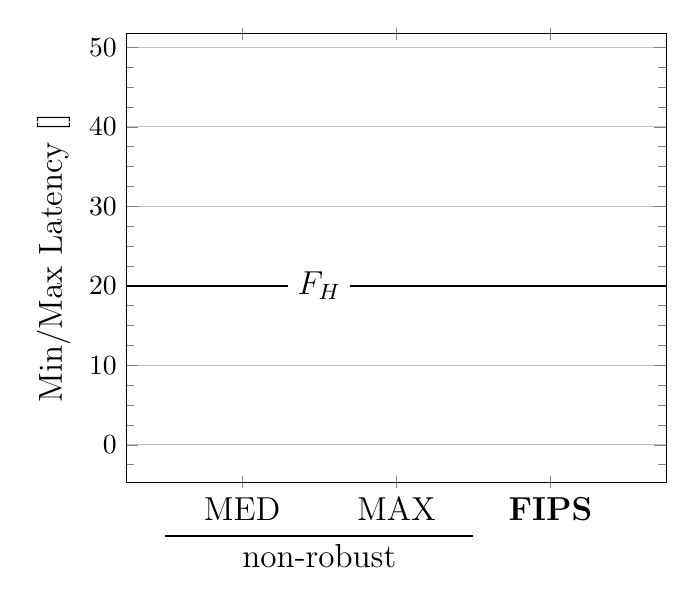
\begin{tikzpicture}
	\begin{axis}[
	      ylabel = {\large Min/Max Latency [\unit{\ms}]},
	      xtick = {1,2,3},
	      xtick align=center, 
	      minor y tick num = 3,
	      enlarge y limits,
	      xmin = 0.25, xmax = 3.75,
	      ymin = 0, ymax = 47,
	      ymajorgrids,
	      xticklabels = {\large MED, \large MAX, \large \textbf{FIPS}},
	      clip=false,
	    ]

	    \draw[thick] (axis cs:0.25,20) -- (axis cs:3.75,20);
	    \node[fill=white] at (axis cs: 1.5,20) {\large $\ete{F_H}$};

	    % CORE_AGV0_00
	    \intervalplt at (1, 4.983, 45.136);
	    \intervalplt at (2, 16.708, 24.55);
	    \intervalplt at (3, 17.918, 18.017);

	    \draw[thick] (axis cs: 0.5,-11.5) -- (axis cs: 2.5,-11.5);
	    \node at (axis cs: 1.5,-14) {\large non-robust};
	\end{axis}
      \end{tikzpicture}
      }
  \end{subfigure}
  \hfill
  \begin{subfigure}{0.48\columnwidth}
    \centering
      \resizebox{\textwidth}{!}{%
	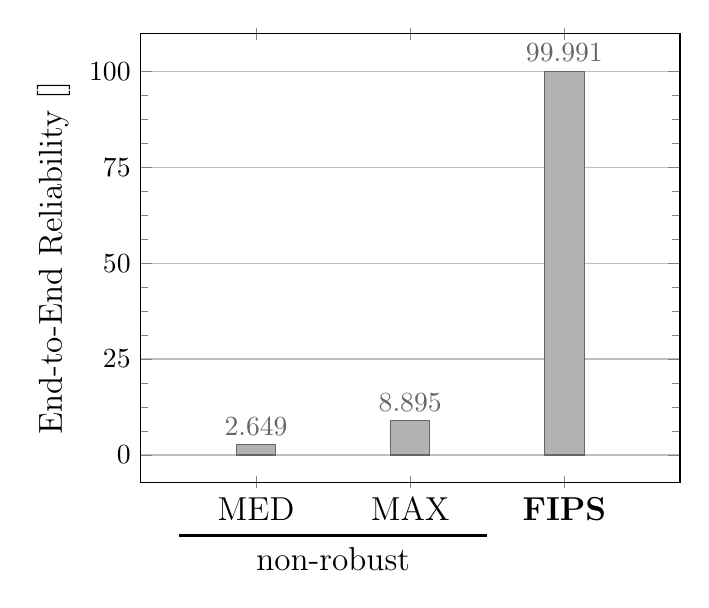
\begin{tikzpicture}
	  \begin{axis}[
		ybar,
		ylabel = {\large End-to-End Reliability [\unit{\percent}]},
		ytick = {0, 25, 50, 75, 100},
		xtick align=center, 
		minor y tick num = 3,
		ymajorgrids,
		enlarge y limits,
		xtick = {1,2,3},
		xmin = 0.25, xmax = 3.75,
		xticklabels = {\large MED, \large MAX, \large \textbf{FIPS}},
		nodes near coords,
		nodes near coords align={vertical},
		nodes near coords style={/pgf/number format/.cd,precision=3},
		clip=false,
	    ]

	      \addplot[black!60,fill=black!30,bar width=0.5cm] coordinates {(1, 2.6491) (2, 8.8948) (3, 99.9914)};

	      \draw[thick] (axis cs: 0.5,-21) -- (axis cs: 2.5,-21);
	      \node at (axis cs: 1.5,-27) {\large non-robust};
	  \end{axis}
	\end{tikzpicture}
      }
  \end{subfigure}
  \caption{Simulation results showing the achieved QoS of $F_H$.} \label{fig:simulation}
\end{figure}



We analyze the behavior of ten high-criticality wireless streams $F_H$ (five per uplink/downlink direction) with requirements $\ete{F_H} = \qty{20}{\ms}$, $\jitter{F_H} = \qty{100}{\us}$, and $\rel{F_H} = \qty{99.99}{\percent}$.
To increase link congestion, we schedule an additional 10~wired streams (five per wired partition) and 80~wireless streams with $\rel{F} = \qty{50}{\percent}$.
The experiments are repeated for one million hypercycles, a simulation time of approx. $\qty{5.6}{h}$.

Fig.~\ref{fig:simulation} shows the achieved QoS guarantees of a representative high-criticality stream $F_H$.
The results clearly show that the observed end-to-end reliability diminishes for both non-robust approaches below $\qty{10}{\percent}$ and is thereby far from the required $\qty{99.99}{\percent}$.
Moreover, the latency results demonstrate that a frame reordering events as in Section~\ref{sec:problem_description} can create a queueing backlog that pushes frames of $F_H$ until after their deadline or even into subsequent hypercycles.
These results therefore underline the need for provable per-stream QoS guarantees, as we provide with FIPS.

% Logs are provided in scalability_results.log
\begin{figure}[b]
  \centering
  \begin{subfigure}{0.48\columnwidth}
    \centering
    \resizebox{\textwidth}{!}{%
    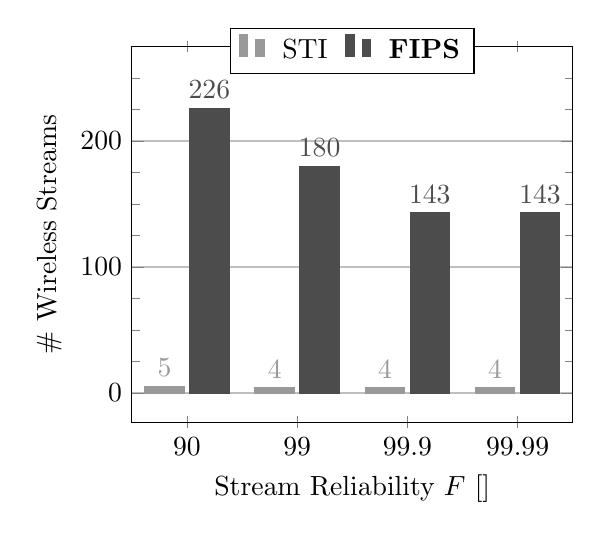
\begin{tikzpicture}
	  \begin{axis}[
		ybar,
		ylabel = {\# Wireless Streams},
		xlabel = {Stream Reliability $\rel{F}$ [$\unit{\percent}$]},
		xtick align=center, 
		minor y tick num = 3,
		ymajorgrids,
		xmin=0.5, xmax=4.5,
		ymax=275,
		xtick = {1,2,3,4},
		xticklabels = {\qty{90}{\percent}, \qty{99}{\percent}, \qty{99.9}{\percent}, \qty{99.99}{\percent}},
		nodes near coords,
		x=1.4cm,
		y=0.016cm,
		nodes near coords align={vertical},
		legend style={at={(0.5,1.05)}, column sep=1ex, anchor=north},
		legend columns=-1,
	    ]
	      \addplot[black!40,fill=black!40,bar width=0.5cm] coordinates {(1, 5) (2, 4) (3, 4) (4, 4)};
	      \addlegendentry{STI}
	      \addplot[black!70,fill=black!70,bar width=0.5cm] coordinates {(1, 226) (2, 180) (3, 143) (4, 143)};
	      \addlegendentry{\textbf{FIPS}}
	  \end{axis}
    \end{tikzpicture}
    }
  \end{subfigure}
  \hfill
  \begin{subfigure}{0.48\columnwidth}
    \centering
    \resizebox{\textwidth}{!}{%
    \begin{tikzpicture}
	  \begin{axis}[
		ylabel = {\# Wireless Streams},
		xlabel = {Jitter $\jitter{F}$ [$\unit{\us}$]},
		xtick align=center, 
		minor y tick num = 3,
		ymajorgrids,
		xmin=-10, xmax=110,
		ymax=275,
		y=0.016cm,
		x=0.045cm,
		legend style={at={(0.44,1.05)}, column sep=1ex, anchor=north},
		legend columns=2,
	    ]
	      \addlegendimage{empty legend}
	      \addlegendentry{\hspace*{-0.75cm}STI}
	      \addlegendimage{empty legend}
	      \addlegendentry{\hspace*{-0.75cm}\textbf{FIPS}}
	      \addplot[black!40,dashed,mark options={black!40,scale=1.2,solid},mark=*] coordinates {(1, 5) (20, 5) (40, 5) (60, 5) (80, 5) (100, 5)};
	      \addlegendentry{$\qty{90}{\percent}$}
	      \addplot[black!70,mark options={black!70,scale=1.2},mark=*] coordinates {(1, 29) (20, 63) (40, 99) (60, 136) (80, 174) (100, 227)};
	      \addlegendentry{$\qty{90}{\percent}$}
	      \addplot[black!40,dashed,mark options={black!40,solid,scale=1.75},mark=triangle*] coordinates {(1, 4) (20, 4) (40, 4) (60, 4) (80, 4) (100, 4)};
	      \addlegendentry{$\qty{99.99}{\percent}$}
	      \addplot[black!70,mark options={black!70,scale=1.75},mark=triangle*] coordinates {(1, 12) (20, 36) (40, 60) (60, 84) (80, 108) (100, 143)};
	      \addlegendentry{$\qty{99.99}{\percent}$}
	  \end{axis}
    \end{tikzpicture}
    }
  \end{subfigure}
  \caption{Scalability results for STI and FIPS. 
    The results on the left are obtained with $\jitter{F} = \qty{100}{\us}$.
  } \label{fig:scalability}
\end{figure}



\subsection{Comparing FIPS with Strict Transmission Isolation} \label{sec:eval:sti}
Next, we analyze the impact of robustness on scalability in the number of schedulable streams.
We compare FIPS to strict transmission isolation (STI) approaches, e.g., as commonly employed in wired TSN~\cite{nwps,Craciunas2016RTNS}.
To constitute a fair comparison, STI configurations are derived using the incremental heuristic of FIPS but restrict batching to one frame per batch.

Fig.~\ref{fig:scalability} shows the maximum number of wireless streams for which STI and FIPS find a feasible TSN configuration.
We consider stream sets that consist of 30 internal streams (15 per wired partition) and 400 wireless streams (200 per up-/downlink direction) with randomly generated paths.
The results show the total number of accepted wireless streams, averaged over 100 stream sets, in dependence of different reliability ($\qty{90}{\percent}$ -- $\qty{99.99}{\percent}$) and jitter ($\qty{1}{\us}$ -- $\qty{100}{\us}$) requirements.

Fig.~\ref{fig:scalability} shows the poor scalability of STI with little to no variation over the different QoS requirements.
This is due to the large 5G packet delay variations that cause STI to reserve egress queues at the DS-TT/NW-TT exclusively for individual frames.
In contrast, FIPS shows an expected downward trend for increasing reliability requirements and an upward trend for increasing jitter allowance. 
Hence, we identify the jitter allowance of streams, which essentially restricts the maximum batch size, as the limiting factor for deploying FIPS at scale.

